\documentclass[11pt]{article}
\usepackage[letterpaper,margin=2cm]{geometry}
\usepackage[english]{babel}
\usepackage[utf8]{inputenc}
\usepackage[T1]{fontenc}
\linespread{1.3}
\parskip=12pt
\parindent=0pt
\usepackage{enumerate}
\usepackage{amsmath}
\usepackage{amsfonts}
\usepackage{graphicx}
\usepackage[section]{placeins}
\usepackage{amsthm}
\usepackage{amssymb}
\usepackage{mathpazo}
\usepackage{booktabs}
\usepackage{float}
\usepackage{listings}

\usepackage[dvipsnames]{xcolor}
\definecolor{slateblue}{RGB}{45, 62, 80}
\definecolor{FGVBlue}{RGB}{0, 114, 188}
\usepackage{hyperref}
\hypersetup{
	colorlinks=true,
	linkcolor=FGVBlue,
	urlcolor=FGVBlue,
	citecolor=FGVBlue,
}

\lstset{language=R, basicstyle=\ttfamily\footnotesize, breaklines=true,
	commentstyle=\color{gray}, keywordstyle=\color{slateblue}\bfseries,
	frame=single, rulecolor=\color{lightgray}, columns=fullflexible, keepspaces=true,
	showstringspaces=false}

% Custom commands
\newcommand{\E}{\mathbb{E}}
\newcommand{\Var}{\mathrm{Var}}
\newcommand{\Cov}{\mathrm{Cov}}
\newcommand{\Prob}{\mathbb{P}}
\newcommand{\symbf}[1]{\boldsymbol{#1}}

\newcounter{problem}
\renewcommand{\theproblem}{\arabic{problem}}
\newcommand{\problem}{
	\stepcounter{problem}
	\section*{Problem \theproblem}
}
\newcommand{\itm}[1]{\par\textbf{#1)}\ }
% Expandable \input, so that table rows can be read inside a tabular
\makeatletter
\newcommand{\tablerows}[1]{\@@input #1 }
\makeatother

\begin{document}
	\begin{center}
		{\LARGE{\textbf{Problem Set II -- Solutions}}}\\
		\vspace{0.2cm}
		Econometrics I - \textcolor{FGVBlue}{FGV EPGE}\\
		Instructor: Raul Guarini Riva \\
		TA: Taric Latif Padovani
	\end{center}

The code for Problems 6 and 7 is in R and is reproduced at the end of each problem. Simulations use \texttt{set.seed(2026)}, so the numbers below are exactly reproducible. The data run from February 1995 to September 2026 ($T=380$ months).

%=====================================================================
\problem

\itm{a}
Since $\cos(t+\theta) = \cos t\cos\theta - \sin t\sin\theta$, the four equally likely values of $\theta$ give
\[
y_t\in\big\{\cos t,\ -\sin t,\ -\cos t,\ \sin t\big\},\qquad\text{each with probability } \tfrac14 .
\]
\emph{Mean.} $\E[y_t] = \frac14(\cos t - \sin t - \cos t + \sin t) = 0$ for every $t$.

\emph{Autocovariances.} Using $\cos A\cos B = \frac12\big[\cos(A-B) + \cos(A+B)\big]$,
\[
\Cov(y_t,y_{t+h}) = \E\big[\cos(t+\theta)\cos(t+h+\theta)\big] = \frac12\cos h + \frac12\E\big[\cos(2t+h+2\theta)\big].
\]
Here $2\theta\in\{0,\pi,2\pi,3\pi\}$ with equal probabilities, and for any $a$, $\cos a + \cos(a+\pi) + \cos(a+2\pi) + \cos(a+3\pi) = \cos a-\cos a+\cos a-\cos a = 0$. So the last expectation is zero and
\[
\gamma_h = \Cov(y_t,y_{t+h}) = \frac12\cos h .
\]
The mean is constant, the variance $\gamma_0=\frac12$ is finite, and the autocovariances depend only on the lag $h$, not on $t$. So $\{y_t\}$ is weakly stationary.

\itm{b}
Strict stationarity requires, in particular, that $y_t$ has the same distribution for every $t$. Compare $t=0$ and $t=1$ (recall $t\in\mathbb Z$):
\[
y_0\in\{1,\,0,\,-1,\,0\},\qquad y_1\in\{\cos 1,\,-\sin 1,\,-\cos 1,\,\sin 1\}\approx\{0.54,\,-0.84,\,-0.54,\,0.84\}.
\]
So $\Prob(y_0=0)=\frac12$, while $\Prob(y_1=0)=0$. The marginal distributions differ, so the process is not strictly stationary. Weak stationarity only looks at the first two moments, and these happen to match; the distributions themselves do not.

\itm{c}
Let $Z\in\{0,1\}$ be the coin flip that fixes the whole path, so $z_t=Z$ for all $t$. Then
\[
\E[z_t] = \E[Z] = \tfrac12,\qquad \E[z_t^2] = \E[Z^2] = \tfrac12,\qquad \Var(z_t) = \tfrac12-\tfrac14 = \tfrac14,
\]
\[
\gamma_h = \Cov(z_t,z_{t+h}) = \Var(Z) = \tfrac14\quad\text{for every } h.
\]
The mean and variance are constant and $\gamma_h$ does not depend on $t$, so $\{z_t\}$ is weakly stationary (it is even strictly stationary).

But every realized path is constant: either $z_t=1$ for all $t$ or $z_t=0$ for all $t$. So, for every $T$,
\[
\bar z_T = \frac1T\sum_{t=1}^Tz_t = Z\in\{0,1\},
\]
which is never equal to, or close to, $\E[z_t]=\frac12$. The time average converges, but to the random variable $Z$, not to the population mean. The process is not mean-ergodic: one path only ever shows one of the two ``worlds,'' and no amount of time-series data reveals the other. Formally, $\gamma_h=\frac14$ does not die out as $h\to\infty$, so observations far apart in time carry no new information.

%=====================================================================
\problem

The lag polynomial factors as
\[
1-1.1z+0.18z^2 = (1-0.9z)(1-0.2z),
\]
with roots $z=1/0.9=10/9$ and $z=1/0.2=5$, both outside the unit circle. So the equation has a unique weakly stationary solution, $y_t = (1-0.9L)^{-1}(1-0.2L)^{-1}\varepsilon_t$, a causal MA($\infty$) in current and past shocks.

\emph{Mean.} There is no constant, so taking expectations gives $\E[y_t](1-1.1+0.18)=0$, that is, $\E[y_t]=0$.

\emph{Autocorrelations.} Write $y_t = \phi_1y_{t-1}+\phi_2y_{t-2}+\varepsilon_t$ with $\phi_1=1.1$ and $\phi_2=-0.18$. Multiplying by $y_{t-k}$, $k\ge1$, and taking expectations (the shock $\varepsilon_t$ is uncorrelated with past $y$'s) gives the Yule--Walker equations
\[
\rho_k = \phi_1\rho_{k-1} + \phi_2\rho_{k-2},\qquad k\ge 1,\qquad \rho_0=1,\ \rho_{-1}=\rho_1 .
\]
For $k=1$: $\rho_1 = \phi_1/(1-\phi_2) = 1.1/1.18 = 55/59\approx0.932$. For $k\ge2$, the recursion has characteristic roots $0.9$ and $0.2$ (the inverses of the lag-polynomial roots), so $\rho_k = A(0.9)^k + B(0.2)^k$. The conditions $\rho_0 = A+B = 1$ and $\rho_1 = 0.9A+0.2B = 55/59$ give
\[
A = \frac{55/59-0.2}{0.7} = \frac{432}{413},\qquad B = 1-A = -\frac{19}{413},
\qquad\text{so}\qquad
\rho_k = \frac{432}{413}(0.9)^k - \frac{19}{413}(0.2)^k,\quad k\ge0 .
\]
\emph{Variance.} Multiplying the equation by $y_t$ and taking expectations, $\gamma_0 = \phi_1\gamma_1 + \phi_2\gamma_2 + \sigma^2$, so
\[
\gamma_0 = \frac{\sigma^2}{1-\phi_1\rho_1-\phi_2\rho_2},\qquad \rho_2 = \phi_1\rho_1+\phi_2 = \frac{1247}{1475}\approx 0.845,
\]
which gives
\[
\gamma_0 = \frac{\sigma^2}{1-1.1\cdot\frac{55}{59}+0.18\cdot\frac{1247}{1475}} = \frac{36875}{4674}\,\sigma^2\approx 7.889\,\sigma^2 .
\]
As a check, the closed form for the variance of an AR(2) gives the same number:
\[
\gamma_0 = \frac{(1-\phi_2)\,\sigma^2}{(1+\phi_2)\left[(1-\phi_2)^2-\phi_1^2\right]} = \frac{1.18\,\sigma^2}{0.82\cdot 0.1824}\approx 7.889\,\sigma^2 .
\]

\emph{Autocovariance function.} For every integer $h$,
\[
\gamma_h = \gamma_0\,\rho_{|h|} = \frac{36875}{4674}\,\sigma^2\left[\frac{432}{413}(0.9)^{|h|} - \frac{19}{413}(0.2)^{|h|}\right].
\]
The root at $0.9$ dominates: the process is very persistent (its variance is almost eight times that of the shock), and the autocorrelations decay roughly like $0.9^h$.

%=====================================================================
\problem

\itm{a}
Write the equation as $\Phi(L)y_t = -0.22+\varepsilon_t$ with $\Phi(z) = 1-0.3z-0.5z^2-0.2z^3$. The coefficients add up to one, so $\Phi(1) = 1-0.3-0.5-0.2 = 0$: $z=1$ is a root, a \emph{unit root}. Dividing by $(1-z)$,
\[
\Phi(z) = (1-z)(1+0.7z+0.2z^2).
\]
(By the Fundamental Theorem of Algebra, $\Phi$ has exactly three roots, and we have found them all.) The quadratic factor has roots $z = \frac{-0.7\pm\sqrt{0.49-0.8}}{0.4} = -1.75\pm1.39i$, with modulus $\sqrt{1/0.2} = \sqrt5\approx2.24$, outside the unit circle. The root $z=1$ lies on the unit circle.

There is no weakly stationary solution. The quickest argument uses the constant. If $y_t$ were weakly stationary with mean $\nu$, taking expectations on both sides would give
\[
\nu = -0.22 + (0.3+0.5+0.2)\,\nu = -0.22+\nu,
\]
that is, $0=-0.22$, a contradiction. (Without the constant the mean equation would be satisfied, but the unit root still rules out a stationary solution: $\Phi(L)$ cannot be inverted, and item b) shows that $y_t$ is the sum of all past changes, whose variance grows without bound.) Since there is no stationary solution, there is no autocovariance function to compute.

\itm{b}
Use the factorization: $(1+0.7L+0.2L^2)(1-L)y_t = -0.22+\varepsilon_t$, and $(1-L)y_t=\Delta y_t$. So
\[
\Delta y_t = -0.22 - 0.7\,\Delta y_{t-1} - 0.2\,\Delta y_{t-2} + \varepsilon_t .
\]
The differences follow an AR(2), so $y_t$ is an ARIMA(2,1,0): an AR(2) in first differences, integrated once. Its lag polynomial $1+0.7z+0.2z^2$ has both roots outside the unit circle (modulus $\sqrt5$), so $\Delta y_t$ has a unique weakly stationary solution, with mean
\[
\E[\Delta y_t] = \frac{-0.22}{1+0.7+0.2} = -\frac{0.22}{1.9}\approx-0.116 .
\]
So $y_t$ drifts down by about $0.116$ per period on average, with stationary fluctuations around that trend: $y_t = y_0 + \sum_{s=1}^t\Delta y_s$ has a mean that changes with $t$ and a variance that grows with $t$.

%=====================================================================
\problem

\itm{a}
If $\lambda=0$ were a root, then $f(0) = a_0 = 0$, contradicting $a_0\neq0$. So $\lambda\neq0$.

\itm{b}
Since $\lambda\neq0$, we can divide $f(\lambda)=0$ by $\lambda^p$:
\[
0 = \frac{f(\lambda)}{\lambda^p} = a_p + a_{p-1}\frac1\lambda + \cdots + a_1\frac1{\lambda^{p-1}} + a_0\frac1{\lambda^p} = g\!\left(\frac1\lambda\right).
\]
So $1/\lambda$ is a root of $g$. In general, $g(x) = x^pf(1/x)$ for $x\ne0$: $g$ is $f$ with its coefficients in reverse order.

\itm{c}
By the Fundamental Theorem of Algebra, $f(x) = a_p\prod_{j=1}^p(x-\lambda_j)$, where $\lambda_1,\dots,\lambda_p$ are its roots (with multiplicity), all nonzero by a). Then
\[
g(x) = x^pf(1/x) = a_p\prod_{j=1}^p(1-\lambda_jx) = a_p\prod_{j=1}^p(-\lambda_j)\,\prod_{j=1}^p\left(x-\frac1{\lambda_j}\right).
\]
So the roots of $g$ are exactly $1/\lambda_1,\dots,1/\lambda_p$, with the same multiplicities (and $g$ has degree $p$, since its leading coefficient is $a_0\neq0$). If $|\lambda_j|>1$ for all $j$, then $|1/\lambda_j|<1$ for all $j$: every root of $g$ lies inside the unit circle. (Item b) alone shows that each $1/\lambda_j$ is a root of $g$; the factorization also shows that $g$ has no other roots.)

%=====================================================================
\problem

\itm{a}
The lag operator does nothing to a constant: $L^k\mu=\mu$. So
\[
\Phi(L)\mu = \mu-\phi_1\mu-\cdots-\phi_p\mu = (1-\phi_1-\cdots-\phi_p)\,\mu = f(1)\,\mu .
\]
Let $c\equiv\psi(L)\mu = \big(\sum_j\psi_j\big)\mu$, also a constant (the sum converges because, as item d) shows, the $\psi_j$ decay geometrically). Applying $\Phi(L)$ and using $\Phi(L)\psi(L)=I$ (lag polynomials commute),
\[
\mu = \Phi(L)\psi(L)\mu = \Phi(L)c = f(1)\,c
\qquad\Longrightarrow\qquad
\psi(L)\mu = \frac{\mu}{1-\phi_1-\cdots-\phi_p}.
\]
The denominator is $f(1)\neq0$, because $z=1$ is on the unit circle and all roots of $f$ lie outside it. This is the mean of the process: $\E[y_t] = \mu/(1-\sum_i\phi_i)$, since $\E[\psi(L)\varepsilon_t]=0$.

\itm{b}
Multiply out, collecting powers of $L$:
\[
\Big(I-\sum_{i=1}^p\phi_iL^i\Big)\Big(\sum_{j=0}^\infty\psi_jL^j\Big)
= \psi_0 I + \sum_{k=1}^\infty\Big(\psi_k - \phi_1\psi_{k-1}-\phi_2\psi_{k-2}-\cdots-\phi_p\psi_{k-p}\Big)L^k,
\]
where $\psi_j=0$ for $j<0$ takes care of the terms with $k<p$ (for instance, the coefficient on $L$ is $\psi_1-\phi_1\psi_0$). For this to equal $I$, the coefficient on $L^0$ must be one and every other coefficient must be zero:
\[
\psi_0 = 1,\qquad \psi_k = \phi_1\psi_{k-1}+\phi_2\psi_{k-2}+\cdots+\phi_p\psi_{k-p},\quad k\ge1 .
\]
So $\psi_1=\phi_1$, $\psi_2=\phi_1^2+\phi_2$, and so on.

\itm{c}
For $k\ge p$ no $\psi_j$ with negative index appears, and the recursion is a linear, homogeneous, $p$th-order difference equation. Trying $\psi_k=r^k$ and dividing by $r^{k-p}$ gives the characteristic equation
\[
r^p-\phi_1r^{p-1}-\phi_2r^{p-2}-\cdots-\phi_{p-1}r-\phi_p = 0 .
\]
This is the polynomial $g$ of Problem 4 built from $f(x) = 1-\phi_1x-\cdots-\phi_px^p$: the coefficients of $f$ are $a_0=1$, $a_i=-\phi_i$, and reversing them gives $a_p+a_{p-1}r+\cdots+a_0r^p = -\phi_p-\phi_{p-1}r-\cdots-\phi_1r^{p-1}+r^p$. Problem 4 applies because $a_0=1\neq0$ and $a_p=-\phi_p\neq0$. All roots of $f$ lie outside the unit circle, so by Problem 4 c) all roots of the characteristic polynomial lie inside it.

\itm{d}
Let $r_1,\dots,r_q$ be the distinct roots of the characteristic polynomial, with multiplicities $d_1,\dots,d_q$ ($\sum d_j=p$). By c), $\rho\equiv\max_j|r_j|<1$. The sequence $(\psi_k)_{k\ge0}$ solves the difference equation for $k\ge p$, and it is pinned down by its first $p$ values, so the standard result gives constants $c_{j,l}$ with
\[
\psi_k = \sum_{j=1}^q\sum_{l=0}^{d_j-1}c_{j,l}\,k^l\,r_j^k,\qquad k\ge0 .
\]
Each term is bounded by $|c_{j,l}|\,k^{p-1}\rho^k$ (for $k\ge1$), so $|\psi_k|\le C\,k^{p-1}\rho^k$ with $C=\sum_{j,l}|c_{j,l}|$, and
\[
\psi_k^2\le C^2\,k^{2(p-1)}\rho^{2k} \equiv a_k .
\]
By the root test, $a_k^{1/k} = C^{2/k}\,\big(k^{1/k}\big)^{2(p-1)}\rho^2\to\rho^2<1$, because $C^{1/k}\to1$ and $k^{1/k}\to1$. So $\sum_ka_k<\infty$, and by comparison $\sum_{i=0}^\infty\psi_i^2<\infty$. (The ratio test works as well: $a_{k+1}/a_k = (1+1/k)^{2(p-1)}\rho^2\to\rho^2<1$.) The polynomial factor $k^{p-1}$, which appears with repeated roots, cannot beat the geometric decay $\rho^k$. In fact, the same argument gives $\sum_i|\psi_i|<\infty$, which justifies the infinite sum in item a).

%=====================================================================
\problem

\itm{a}
\begin{itemize}
	\item \textbf{IPCA} (\'Indice Nacional de Pre\c{c}os ao Consumidor Amplo) is computed by IBGE. It measures the change in the cost of a basket of goods and services bought by urban households with incomes between 1 and 40 minimum wages, in the main metropolitan areas. It is a pure consumer price index, and it is the official target of the Central Bank's inflation-targeting regime.
	\item \textbf{IGP-M} (\'Indice Geral de Pre\c{c}os -- Mercado) is computed by FGV. It is a weighted average of three indices: producer (wholesale) prices, IPA, with 60\% of the weight; consumer prices, IPC, with 30\%; and construction costs, INCC, with 10\%. Because most of its weight is on producer prices, many of them commodities and tradable goods, it reacts strongly to the exchange rate and to commodity prices. It is widely used to index contracts, such as rents and some regulated prices.
\end{itemize}
In short, IPCA measures the cost of living of households; IGP-M is a broader measure of prices along the production chain, closer to the prices of tradables.

\itm{b}
Figure~\ref{fig:p6series} plots both series.

\begin{figure}[H]
	\centering
	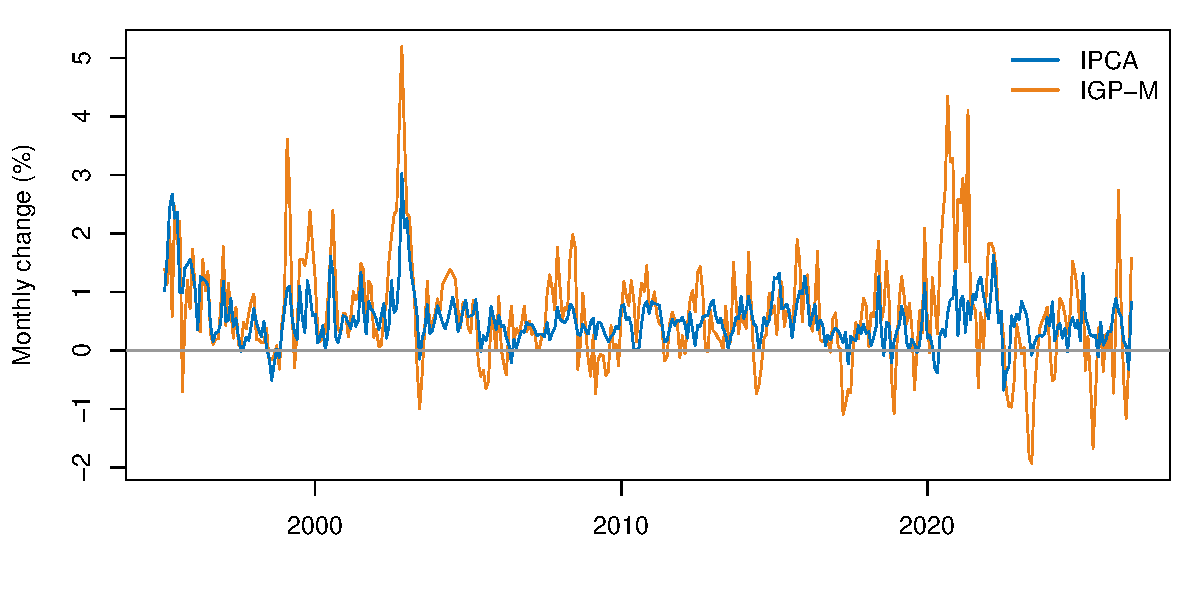
\includegraphics[width=0.9\linewidth]{figures/p6_series.pdf}
	\caption{Monthly changes in IPCA and IGP-M (\%), February 1995 to September 2026.}
	\label{fig:p6series}
\end{figure}

\itm{c}
Table~\ref{tab:p6} reports the sample moments, using the definitions in the problem set (dividing by $T$). The sample means are $0.531\%$ per month for IPCA and $0.644\%$ for IGP-M, and the variances are $0.206$ and $0.829$ (standard deviations of $0.454$ and $0.910$ percentage points). IGP-M is by far the more volatile series: its variance is four times that of IPCA. This fits its composition: the large weight on wholesale and commodity prices passes exchange-rate and commodity shocks through almost immediately, as in the big IGP-M spikes of 2002 and 2020--21.

\begin{table}[H]
	\centering
	\small
	\begin{tabular}{rrrrrrr}
		\toprule
		& \multicolumn{2}{c}{IPCA} & \multicolumn{2}{c}{IGP-M} & \multicolumn{2}{c}{IPCA, seasonally adjusted} \\
		\cmidrule(lr){2-3}\cmidrule(lr){4-5}\cmidrule(lr){6-7}
		$h$ & $\hat\gamma_h$ & $\hat\rho_h$ & $\hat\gamma_h$ & $\hat\rho_h$ & $\hat\gamma_h$ & $\hat\rho_h$ \\
		\midrule
		\tablerows{tables/p6_autocov.tex}
		\bottomrule
	\end{tabular}
	\caption{Sample autocovariances and autocorrelations. The row $h=0$ gives the variances. The last two columns are for $z_t$ in item e)(iv).}
	\label{tab:p6}
\end{table}

\itm{d}
Figure~\ref{fig:p6acf} shows the sample autocorrelations. The dashed lines are $\pm1.96/\sqrt T=\pm0.10$, the band we would expect for i.i.d.\ data.

\begin{figure}[H]
	\centering
	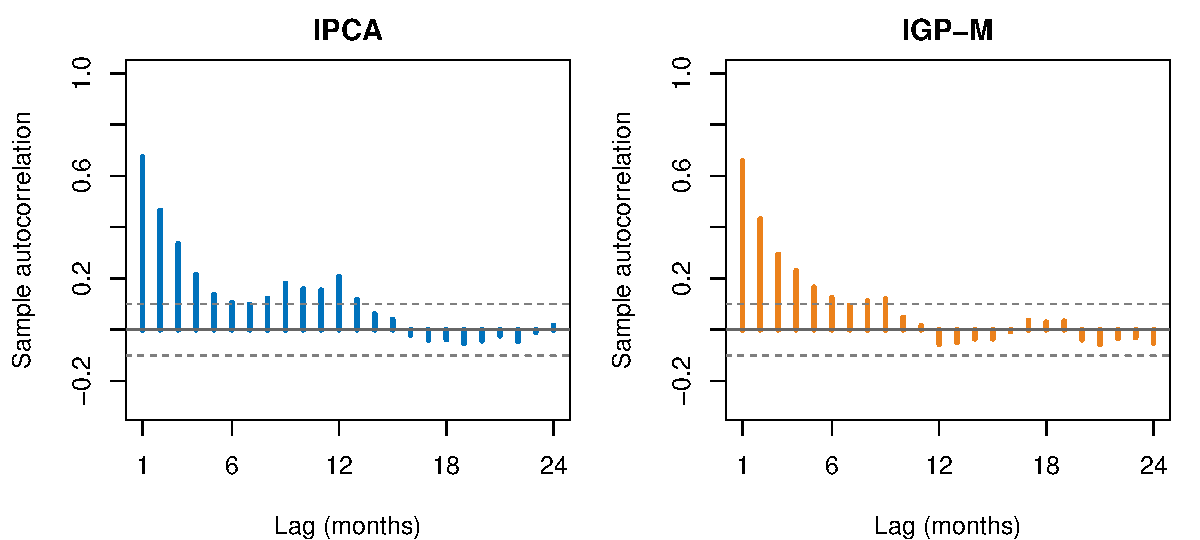
\includegraphics[width=0.95\linewidth]{figures/p6_acf.pdf}
	\caption{Sample autocorrelation functions, lags 1 to 24.}
	\label{fig:p6acf}
\end{figure}

Both series are persistent at short horizons, with almost the same first-order autocorrelation ($0.67$ for IPCA, $0.66$ for IGP-M), and in both the autocorrelations decay roughly geometrically. The difference is at medium horizons. IGP-M's autocorrelations fall to about $0.05$ by lag 10 and are slightly negative after a year: its shocks (exchange rate, commodities) are large but short-lived, and are partly reversed. IPCA's autocorrelations stay between $0.10$ and $0.20$ up to lag 13, and rise again at lag 12 ($0.21$, against $0.15$ at lag 11). So IPCA is more persistent: once consumer inflation picks up, it stays up for longer, consistent with inertia from indexation and slowly adjusting services prices. The bump at lag 12 is the first sign of seasonality.

\itm{e}
\textbf{(i)} Figure~\ref{fig:p6months} plots the average change in each calendar month.

\begin{figure}[H]
	\centering
	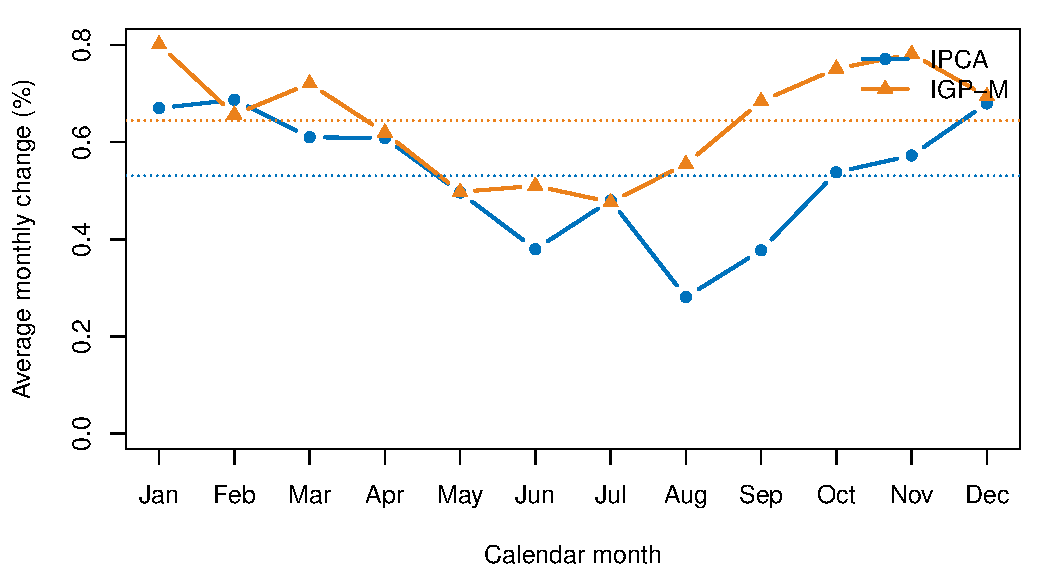
\includegraphics[width=0.75\linewidth]{figures/p6_months.pdf}
	\caption{Average monthly change by calendar month. The dotted lines are the overall means.}
	\label{fig:p6months}
\end{figure}

For IPCA, December, January and February stand out at the top (about $0.67$--$0.69\%$ a month), while June to September are at the bottom (August is the lowest month, at $0.28\%$, against an overall mean of $0.53\%$). Plausible economic reasons: school fees and other education prices are readjusted at the start of the school year (February); many public transport fares and other administered prices are readjusted in January; food prices tend to rise in the rainy season, around the turn of the year, and fall in the middle of the year, with the harvest; and December has holiday-season demand (food, airfares). IGP-M also has a seasonal pattern, but a less clear one ($0.48$--$0.80\%$, highest in January and in October--November), and its large non-seasonal shocks dominate.

\textbf{(ii)} Since $x_t$ has mean zero,
\[
\E[y_t] = s_{m(t)} + \E[x_t] = s_{m(t)} .
\]
The $s_m$'s are not all equal, so there are months $m\neq m'$ with $s_m\neq s_{m'}$, and then $\E[y_t]\neq\E[y_{t'}]$ for any $t$, $t'$ in those calendar months. The condition that fails is the constant mean. The second moments are fine: $s_{m(t)}$ is not random, so $\Var(y_t)=\Var(x_t)$ and $\Cov(y_t,y_{t+h}) = \Cov(x_t,x_{t+h}) = \gamma^x_h$, which depend only on $h$. Seasonality of this kind is a nonstationarity in the mean only.

\textbf{(iii)} Let $c_h\equiv\frac1{12}\sum_{m=1}^{12}(s_m-\bar s)(s_{m+h}-\bar s)$, with the month index wrapping around. Since $y_t = s_{m(t)}$ repeats every 12 months, the sequence $a_t\equiv(s_{m(t)}-\bar s)(s_{m(t+h)}-\bar s)$ also repeats every 12 months, and each block of 12 consecutive terms adds up to $12c_h$.

\emph{First, the sample mean converges to $\bar s$.} $\sum_{t=1}^Ty_t$ is $\lfloor T/12\rfloor$ full years, each adding up to $12\bar s$, plus at most 11 extra terms, each bounded by $S\equiv\max_m|s_m|$. So $|\bar y_T-\bar s|\le 2\cdot 11\,S/T\to0$.

\emph{Second, replace $\bar y_T$ by $\bar s$.} Write $y_t-\bar y_T = (s_{m(t)}-\bar s) - (\bar y_T-\bar s)$ and expand:
\[
\hat\gamma_h = \frac1T\sum_{t=1}^{T-h}a_t \;-\; (\bar y_T-\bar s)\,\frac1T\sum_{t=1}^{T-h}\Big[(s_{m(t)}-\bar s)+(s_{m(t+h)}-\bar s)\Big] \;+\; \frac{T-h}{T}(\bar y_T-\bar s)^2 .
\]
The sums in the second term are bounded by $2T\cdot 2S$, so the second and third terms are bounded by a multiple of $|\bar y_T-\bar s|$ and go to zero.

\emph{Third, the main term.} The $T-h$ terms of $\sum_{t=1}^{T-h}a_t$ form $\lfloor (T-h)/12\rfloor$ full blocks, each adding up to $12c_h$, plus at most 11 extra terms, each bounded by $4S^2$. So
\[
\frac1T\sum_{t=1}^{T-h}a_t = \frac{12\lfloor (T-h)/12\rfloor}{T}\,c_h + O\!\left(\frac1T\right)\ \longrightarrow\ c_h\qquad(T\to\infty,\ h \text{ fixed}).
\]
Hence $\hat\gamma_h\to c_h = \frac1{12}\sum_{m=1}^{12}(s_m-\bar s)(s_{m+h}-\bar s)$.

At $h = 12,24,36,\dots$ we have $s_{m+h}=s_m$, so
\[
c_{12} = c_{24} = \cdots = \frac1{12}\sum_{m=1}^{12}(s_m-\bar s)^2 = c_0 > 0,
\]
the variance of the seasonal pattern, and the sample autocorrelation $c_{12k}/c_0$ equals one. The reason: twelve months later the seasonal component is exactly the same, so a seasonal series is perfectly correlated with itself at yearly lags, at every horizon. With $x_t$ switched back on, the cross terms between the deterministic $s_{m(t)}$ and the mean-zero $x_t$ average out, and $\hat\gamma_h$ converges to $c_h+\gamma^x_h$. Since $\gamma^x_h\to0$, the autocorrelation function has spikes at $12, 24, 36,\dots$ that never die out. These spikes are how seasonality shows up in a correlogram.

\textbf{(iv)} Let $z_t = y_t-\hat s_{m(t)}$ for IPCA. Figure~\ref{fig:p6acfsa} compares the two autocorrelation functions, and the last columns of Table~\ref{tab:p6} give the numbers.

\begin{figure}[H]
	\centering
	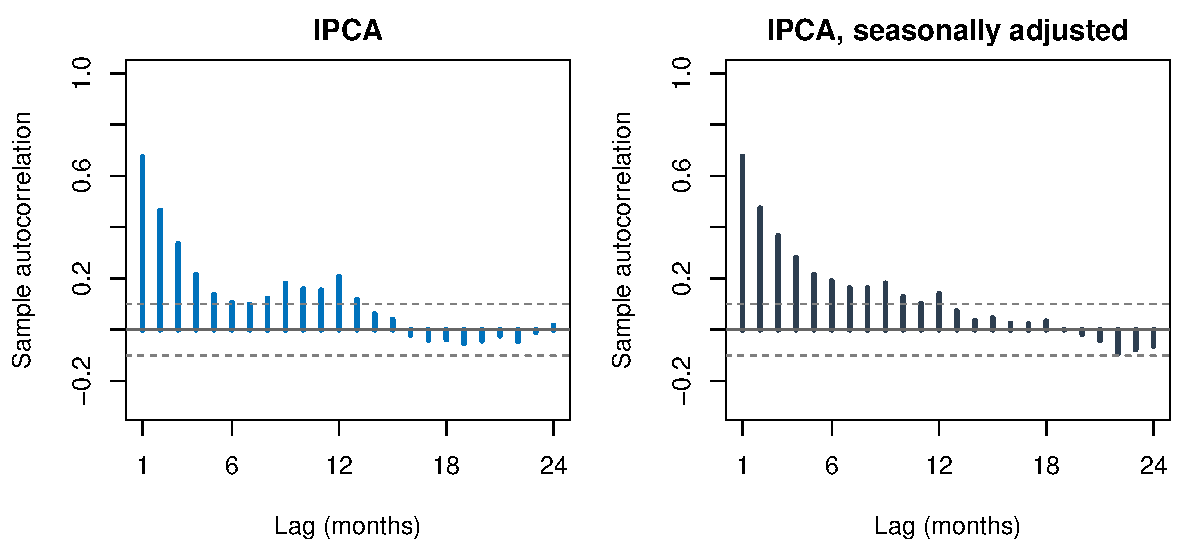
\includegraphics[width=0.95\linewidth]{figures/p6_acf_sa.pdf}
	\caption{Sample autocorrelations of IPCA, before and after removing the calendar-month means.}
	\label{fig:p6acfsa}
\end{figure}

\begin{itemize}
	\item \emph{Item c) for $z_t$.} The mean of $z_t$ is exactly zero: within each calendar month we subtract that month's sample mean. The variance falls from $0.206$ to $0.190$: the fixed seasonal pattern accounts for about $8\%$ of the variance of monthly IPCA.
	\item \emph{Item e)(i) for $z_t$.} The calendar-month averages of $z_t$ are all exactly zero, again by construction, so the plot is a flat line at zero (not shown).
	\item \emph{Item d) for $z_t$.} The spike at lag 12 shrinks but does not disappear. Before, $\hat\rho_{12}=0.21$ stood about $0.07$ above the average of its neighbours ($0.15$ at lag 11, $0.12$ at lag 13). After, $\hat\rho_{12}=0.14$ stands about $0.05$ above them ($0.10$ and $0.07$). Two reasons it survives: the seasonal pattern itself changes over three decades, and subtracting one fixed set of month means removes only the average pattern; and sampling noise is of order $\pm0.10$. Outside the yearly lags, the autocorrelations of $z_t$ are slightly higher than those of $y_t$ at lags 3--9: removing the seasonal means removes some movements that were working against persistence.
\end{itemize}

\itm{f}
Treating monthly inflation as stationary is a strong assumption, and the data give several reasons for doubt:
\begin{itemize}
	\item \textbf{Seasonality.} The mean depends on the calendar month, which by item e)(ii) violates weak stationarity. This one is easy to deal with, by removing the seasonal means or adding month dummies.
	\item \textbf{Changes in the level.} Average monthly IPCA was $0.73\%$ in 1995--99, $0.54\%$ in 2000--09, $0.47\%$ in 2010--19 and $0.46\%$ in 2020--26. The sample starts in the year after the Real Plan and spans the adoption of inflation targeting in 1999, so the early years belong to a different monetary regime.
	\item \textbf{Changes in volatility.} The standard deviation of IPCA went from $0.67$ (1995--99) to $0.32$ (2010--19) and back up to $0.42$ (2020--26); that of IGP-M doubled from the 2010s to the 2020s ($0.61$ to $1.25$). Episodes such as 2002--03 and 2020--22 look like bursts, not like draws from a single distribution with constant variance.
\end{itemize}
On the other hand, the autocorrelations decay fairly fast, unlike those of a unit-root process, and the series do not drift away. A reasonable conclusion: a stationary model is a useful approximation for seasonally adjusted inflation within a stable monetary regime (say, since 1999), but over the full sample the mean and variance are not plausibly constant, and inference that relies on stationarity, such as the confidence intervals of Problem 7 f), should be read with that in mind.

\lstinputlisting[caption={Problem 6 (\texttt{code/p6\_inflation.R})}]{code/p6_inflation.R}

%=====================================================================
\problem

\itm{a}
\textbf{(i)} Let $S_T=\sum_{t=1}^Ty_t$. By bilinearity of the covariance and stationarity,
\[
\Var(S_T) = \sum_{t=1}^T\sum_{s=1}^T\Cov(y_t,y_s) = \sum_{t=1}^T\sum_{s=1}^T\gamma_{t-s}.
\]
Group the pairs by $h=t-s\in\{-(T-1),\dots,T-1\}$. For a given $h\ge0$, the pairs are $(t,s)=(h+1,1),(h+2,2),\dots,(T,T-h)$: there are $T-h$ of them; for $h<0$, by symmetry, there are $T-|h|$. So
\[
\Var\big(\sqrt T\,\bar y_T\big) = \frac1T\Var(S_T) = \frac1T\sum_{h=-(T-1)}^{T-1}(T-|h|)\,\gamma_h = \sum_{h=-(T-1)}^{T-1}\left(1-\frac{|h|}T\right)\gamma_h .
\]

\textbf{(ii)} With $\gamma_h=\phi_1^{|h|}\gamma_0$,
\[
\Var\big(\sqrt T\,\bar y_T\big) = \gamma_0\sum_{|h|<T}\phi_1^{|h|} - \frac{\gamma_0}T\sum_{|h|<T}|h|\,\phi_1^{|h|}.
\]
The first sum converges, since $|\phi_1|<1$, to $1+2\sum_{h\ge1}\phi_1^h = 1+\frac{2\phi_1}{1-\phi_1} = \frac{1+\phi_1}{1-\phi_1}$. The second sum is bounded by $2\sum_{h\ge1}h|\phi_1|^h = \frac{2|\phi_1|}{(1-|\phi_1|)^2}<\infty$, so divided by $T$ it goes to zero. Hence
\[
\Var\big(\sqrt T\,\bar y_T\big)\ \longrightarrow\ \omega^2 = \gamma_0\,\frac{1+\phi_1}{1-\phi_1} = \frac{\sigma^2}{1-\phi_1^2}\cdot\frac{1+\phi_1}{1-\phi_1} = \frac{\sigma^2}{(1-\phi_1)^2},
\]
using $\gamma_0=\sigma^2/(1-\phi_1^2)$ and $1-\phi_1^2=(1-\phi_1)(1+\phi_1)$. The quantity $\omega^2$ is the \emph{long-run variance}.

\textbf{(iii)} $\omega^2>\gamma_0$ if and only if $\frac{1+\phi_1}{1-\phi_1}>1$, that is, $\phi_1>0$. With positive autocorrelation, neighbouring observations move together, so each new observation brings less new information than an independent draw would, and the sample mean is more variable than under i.i.d.\ sampling. With $\phi_1<0$, deviations tend to be undone the next period and partly cancel in the average, so $\omega^2<\gamma_0$.

\itm{b}
\textbf{(i)} Conditional on the data, each $y^*_t$ takes each of the values $y_1,\dots,y_T$ with probability $1/T$. So
\[
\E^*[y^*_t] = \frac1T\sum_{s=1}^Ty_s = \bar y_T,\qquad \Var^*(y^*_t) = \frac1T\sum_{s=1}^T(y_s-\bar y_T)^2 = \hat\gamma_0 .
\]

\textbf{(ii)} By construction, the draws $y^*_1,\dots,y^*_T$ are independent conditional on the data: the index drawn for position $t$ has nothing to do with the index drawn for position $s$. Independent variables are uncorrelated, so $\Cov^*(y^*_t,y^*_s)=0$. The time ordering of the data plays no role in the resampling, so the bootstrap has no way of knowing that $y_t$ and $y_{t+1}$ were neighbours. Then
\[
\Var^*\big(\sqrt T\,\bar y^*_T\big) = \frac1T\sum_{t=1}^T\Var^*(y^*_t) = \hat\gamma_0 .
\]

\textbf{(iii)} The Gaussian AR(1) is strictly stationary and ergodic with $\E[y_t^2]<\infty$, so by the ergodic theorem $\bar y_T\xrightarrow{p}\nu$ and $\frac1T\sum_ty_t^2\xrightarrow{p}\E[y_t^2]$. Hence
\[
\Var^*\big(\sqrt T\,\bar y^*_T\big) = \hat\gamma_0 = \frac1T\sum_{t=1}^Ty_t^2-\bar y_T^2\ \xrightarrow{p}\ \E[y_t^2]-\nu^2 = \gamma_0 .
\]
The bootstrap estimates $\gamma_0$, while the variance we need is $\omega^2 = \gamma_0\frac{1+\phi_1}{1-\phi_1} = \sum_h\gamma_h$. It throws away all the autocovariances $\gamma_h$, $h\neq0$: the serial dependence of the data. It is right only when $\phi_1=0$.

\textbf{(iv)} If $\sqrt T R^*_T$ is approximately $N(0,\gamma_0)$ given the data, its quantiles are $\sqrt T q^*_\alpha\approx z_\alpha\sqrt{\gamma_0}$, with $z_\alpha=\Phi^{-1}(\alpha)$. So $q^*_{0.975}\approx1.96\sqrt{\gamma_0/T}$ and $q^*_{0.025}\approx-1.96\sqrt{\gamma_0/T}$, and the interval is
\[
\left[\bar y_T-q^*_{0.975},\ \bar y_T-q^*_{0.025}\right]\approx\left[\bar y_T-1.96\sqrt{\gamma_0/T},\ \bar y_T+1.96\sqrt{\gamma_0/T}\right].
\]
It covers $\nu$ when $|\bar y_T-\nu|\le1.96\sqrt{\gamma_0/T}$. Dividing by $\omega/\sqrt T$,
\[
\Prob\left(\left|\frac{\sqrt T(\bar y_T-\nu)}{\omega}\right|\le1.96\,\frac{\sqrt{\gamma_0}}{\omega}\right)\ \longrightarrow\ 2\,\Phi\!\left(1.96\sqrt{\frac{\gamma_0}{\omega^2}}\right)-1 = 2\,\Phi\!\left(1.96\sqrt{\frac{1-\phi_1}{1+\phi_1}}\right)-1,
\]
because $\sqrt T(\bar y_T-\nu)/\omega\xrightarrow{d}N(0,1)$ and, for $Z\sim N(0,1)$, $\Prob(|Z|\le c) = 2\Phi(c)-1$. (In practice the bootstrap quantiles use $\hat\gamma_0$, which converges to $\gamma_0$, so the limit is the same by Slutsky's theorem.)

\textbf{(v)} The formula gives:

\begin{table}[H]
	\centering
	\begin{tabular}{lcccc}
		\toprule
		$\phi_1$ & $-0.5$ & $0$ & $0.5$ & $0.9$ \\
		\midrule
		$\gamma_0/\omega^2 = (1-\phi_1)/(1+\phi_1)$ & $3$ & $1$ & $1/3$ & $1/19$ \\
		Limiting coverage & 99.9\% & 95.0\% & 74.2\% & 34.7\% \\
		\bottomrule
	\end{tabular}
\end{table}

With $\phi_1=-0.5$ the interval is too wide (it overstates the uncertainty by a factor $\sqrt3$); with $\phi_1=0$ it is right; with $\phi_1=0.5$ and $0.9$ it is too narrow, badly so for $\phi_1=0.9$, where it is $\sqrt{19}\approx4.4$ times shorter than it should be.

\itm{c}
With $\mu=0$, $\sigma^2=1$, $T=200$, $M=500$ samples and $B=499$:

\begin{table}[H]
	\centering
	\begin{tabular}{lcccc}
		\toprule
		$\phi_1$ & Coverage & Formula from b)(iv) & Average width & Width with the correct variance \\
		\midrule
		$-0.5$ & 100.0\% & 99.9\% & 0.320 & 0.185 \\
		$0$ & 96.2\% & 95.0\% & 0.275 & 0.277 \\
		$0.5$ & 73.2\% & 74.2\% & 0.316 & 0.554 \\
		$0.9$ & 36.6\% & 34.7\% & 0.592 & 2.772 \\
		\bottomrule
	\end{tabular}
\end{table}

The last column is $2\cdot1.96\,\omega/\sqrt T$, the width the interval would have if it used the long-run variance $\omega^2=1/(1-\phi_1)^2$. The simulated coverage matches the formula up to Monte Carlo noise: with $M=500$, the standard error of a coverage rate $p$ is $\sqrt{p(1-p)/500}$, about $1$ point near $95\%$ and $2$ points near $50\%$--$75\%$. The i.i.d.\ bootstrap is fine only when $\phi_1=0$. For $\phi_1=0.9$ its interval is less than a quarter as wide as it should be, and it misses the true mean almost two times in three.

\emph{Why draw $y_1$ from the stationary distribution?} The calculations in a) and b) assume that the sample comes from the stationary process, so that $\Var(y_t)=\gamma_0$ and $\Cov(y_t,y_{t+h})=\gamma_h$ for every $t$, starting at $t=1$. If we started at, say, $y_1=0$, then $\Var(y_t) = \sigma^2(1-\phi_1^{2(t-1)})/(1-\phi_1^2)$ would start at zero and approach $\gamma_0$ only gradually; with $\phi_1=0.9$, it takes a few dozen periods. The first part of each sample would come from a different, nonstationary process, which is not the one we want to study. Drawing $y_1\sim N(\nu,\gamma_0)$ makes the whole path stationary from the start (the alternative is to simulate a long ``burn-in'' and discard it).

\itm{d}
\textbf{(i)} Figure~\ref{fig:p7iid} shows the IPCA series and one i.i.d.\ bootstrap sample, on the same axes.

\begin{figure}[H]
	\centering
	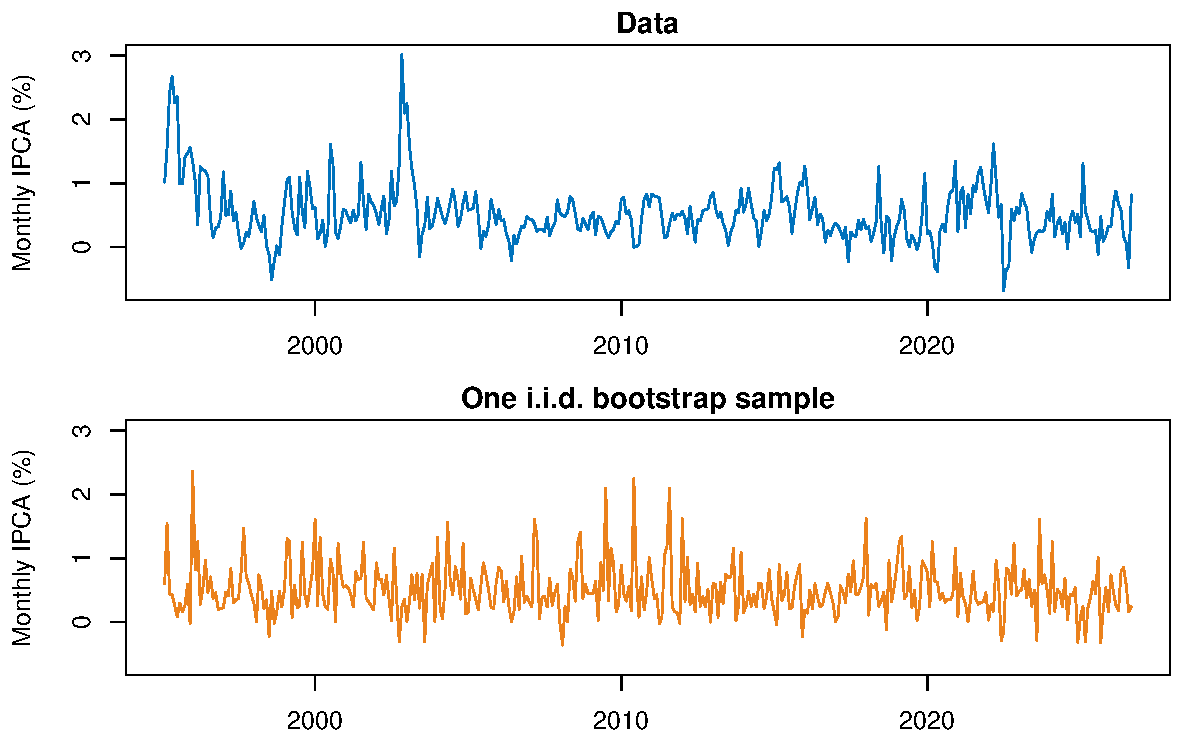
\includegraphics[width=0.9\linewidth]{figures/p7_iid_sample.pdf}
	\caption{Monthly IPCA and one i.i.d.\ bootstrap sample of it.}
	\label{fig:p7iid}
\end{figure}

The bootstrap sample has the same values (the same histogram), but it has lost the time ordering. In the data, high-inflation months come in runs (1995, 2002--03, 2015--16, 2021--22) and calm months follow calm months. In the bootstrap sample, the high values are scattered at random across the three decades and every month is unrelated to the previous one. The persistence, the episodes, and the gradual decline in the level are all gone; so is the seasonality.

\textbf{(ii)} In the data, $\hat\rho_1 = 0.674$. Across $B=999$ i.i.d.\ bootstrap samples, $\hat\rho^*_1$ has mean $-0.002$ and standard deviation $0.053$, and its largest value is $0.216$ (Figure~\ref{fig:p7rho}). The value in the data is more than twelve bootstrap standard deviations away from the center: no bootstrap sample comes anywhere near it.

\begin{figure}[H]
	\centering
	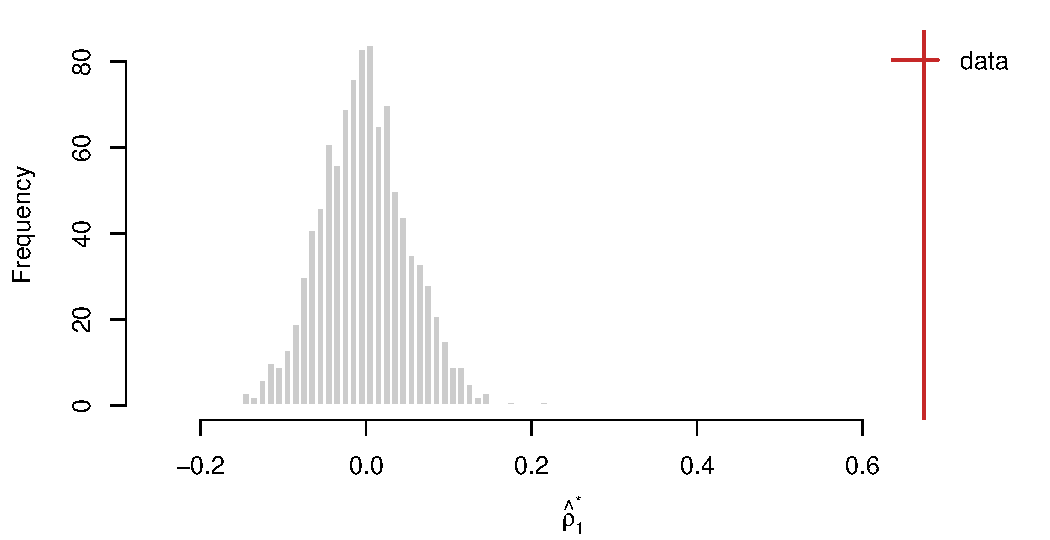
\includegraphics[width=0.7\linewidth]{figures/p7_rho_star.pdf}
	\caption{First-order sample autocorrelation in 999 i.i.d.\ bootstrap samples of IPCA, and in the data.}
	\label{fig:p7rho}
\end{figure}

\textbf{(iii)} Given the data, the $y^*_t$'s are i.i.d.\ draws from $\hat P_T$, so in the bootstrap world $\Cov^*(y^*_t,y^*_{t+1})=0$: the ``true'' first-order autocorrelation is exactly zero. $\hat\rho^*_1$ is the sample autocorrelation of an i.i.d.\ sample, which is centered near zero (its mean is about $-1/T$) with standard deviation about $1/\sqrt T = 0.051$, just what we see. The bootstrap reproduces the distribution of $\hat\rho_1$ \emph{for an independent series}, not for IPCA. Any statistic that depends on the order of the observations, such as an autocorrelation or the variance of a mean under dependence, is estimated as if there were no dependence at all.

\itm{e}
\textbf{(i)} With $b=1$, $k=\lceil T/1\rceil = T$ blocks, each consisting of the single observation $y_{I_j}$, with $I_j$ uniform on $\{1,\dots,T\}$ and independent across $j$. So $y^*_j = y_{I_j}$, $j=1,\dots,T$: $T$ independent draws from the empirical distribution, which is the i.i.d.\ bootstrap.

\textbf{(ii)} The $t$-th bootstrap observation is in block $j=\lceil t/b\rceil$, at offset $r = t-(j-1)b-1\in\{0,\dots,b-1\}$, so $y^*_t = y_{((I_j+r-1)\bmod T)+1}$. Since $I_j$ is uniform on $\{1,\dots,T\}$, so is $((I_j+r-1)\bmod T)+1$: shifting a uniform index by a fixed amount, modulo $T$, just permutes $\{1,\dots,T\}$. Hence each $y^*_t$, on its own, is a uniform draw from $\{y_1,\dots,y_T\}$, $\E^*[y^*_t]=\bar y_T$, and $\E^*[\bar y^*_T] = \frac1T\sum_t\E^*[y^*_t] = \bar y_T$.

The circular extension is used exactly here. Without it (blocks starting only at $1,\dots,T-b+1$, the ``moving block'' bootstrap), observations near the two ends of the sample would appear in fewer blocks than those in the middle (the first observation in only one), so $y^*_t$ would not be uniform on the data and $\E^*[\bar y^*_T]$ would differ from $\bar y_T$. Wrapping the data around a circle makes every observation appear in exactly $b$ of the $T$ possible blocks.

\textbf{(iii)} It depends on whether $t$ and $t+1$ fall in the same block.
\begin{itemize}
	\item If $t$ is not a multiple of $b$, they are consecutive observations of the same block: $(y^*_t,y^*_{t+1}) = (y_s,y_{s+1})$ with $s$ uniform (and $y_{T+1}=y_1$). Using item ii),
	\[
	\Cov^*(y^*_t,y^*_{t+1}) = \frac1T\sum_{s=1}^T y_sy_{s+1}-\bar y_T^2 = \frac1T\sum_{s=1}^T(y_s-\bar y_T)(y_{s+1}-\bar y_T)\equiv\tilde\gamma_1,
	\]
	the circular version of $\hat\gamma_1$ (it adds the single term $(y_T-\bar y_T)(y_1-\bar y_T)/T$). So $y^*_t$ and $y^*_{t+1}$ are correlated, roughly as in the data.
	\item If $t$ is a multiple of $b$, $y^*_t$ is the last observation of one block and $y^*_{t+1}$ the first of the next. The blocks start at independent points, so $\Cov^*(y^*_t,y^*_{t+1})=0$.
\end{itemize}
So the answer depends on $t$: the bootstrap series is not stationary. It reproduces the dependence within blocks and breaks it at every block boundary. A share $(b-1)/b$ of adjacent pairs keeps its correlation, which is why longer blocks keep more of the dependence.

\textbf{(iv)} The same $M=500$ samples per $\phi_1$ are used for every block length, with $B=499$. Coverage of the nominal $95\%$ interval:

\begin{table}[H]
	\centering
	\small
	\begin{tabular}{lcccccccccc}
		\toprule
		& \multicolumn{10}{c}{Block length $b$} \\
		\cmidrule(lr){2-11}
		$\phi_1$ & 1 & 2 & 3 & 5 & 10 & 20 & 30 & 50 & 75 & 100 \\
		\midrule
		\tablerows{tables/p7_coverage.tex}
		\bottomrule
	\end{tabular}
\end{table}

The code also runs $\phi_1=0$ as a benchmark without dependence: its coverage is $95$--$96\%$ for $b\le10$ and then falls, to $93.4\%$ at $b=20$, $86.8\%$ at $b=50$ and $76.4\%$ at $b=100$. Figure~\ref{fig:p7cbb} plots coverage and average width.

\begin{figure}[H]
	\centering
	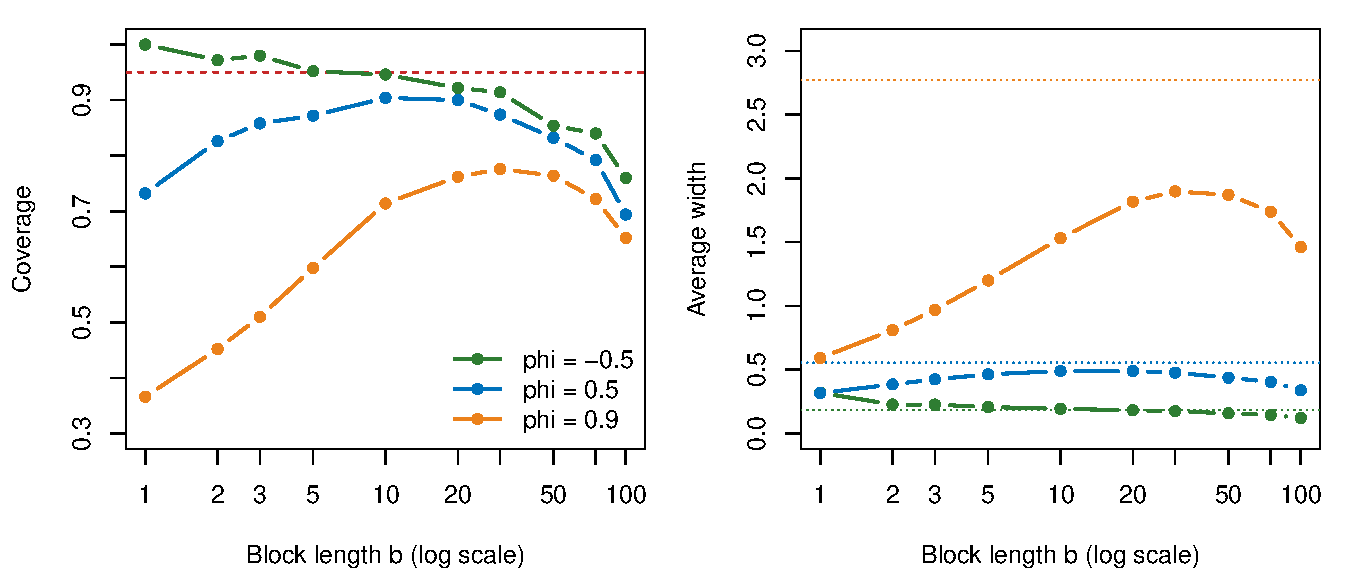
\includegraphics[width=\linewidth]{figures/p7_coverage_width.pdf}
	\caption{Circular block bootstrap: coverage (left; the dashed line is $95\%$) and average width (right; the dotted lines are the widths $2\cdot1.96\,\omega/\sqrt T$ that use the correct long-run variance) as functions of the block length.}
	\label{fig:p7cbb}
\end{figure}

To read these results, it helps to know what the circular block bootstrap estimates. When $b$ divides $T$, $\bar y^*_T$ is the average of $k=T/b$ independent block means, and a calculation like the one in a)(i) gives
\[
\Var^*\big(\sqrt T\,\bar y^*_T\big) = \sum_{|h|<b}\left(1-\frac{|h|}{b}\right)\tilde\gamma_h,
\]
where $\tilde\gamma_h$ are the circular sample autocovariances. Compare with $\omega^2=\sum_h\gamma_h$: the block bootstrap keeps the autocovariances up to lag $b-1$, with weights that fall linearly, and drops the rest. Replacing $\tilde\gamma_h$ by the true $\gamma_h$, the share of $\omega^2$ that it captures is:

\begin{table}[H]
	\centering
	\small
	\begin{tabular}{lcccccccccc}
		\toprule
		$\phi_1$ & 1 & 2 & 3 & 5 & 10 & 20 & 30 & 50 & 75 & 100 \\
		\midrule
		$-0.5$ & 3.000 & 1.500 & 1.500 & 1.275 & 1.133 & 1.067 & 1.044 & 1.027 & 1.018 & 1.013 \\
		$0.5$ & 0.333 & 0.500 & 0.611 & 0.742 & 0.867 & 0.933 & 0.956 & 0.973 & 0.982 & 0.987 \\
		$0.9$ & 0.053 & 0.100 & 0.144 & 0.224 & 0.383 & 0.584 & 0.698 & 0.812 & 0.874 & 0.905 \\
		\bottomrule
	\end{tabular}
\end{table}

This ratio moves toward one as $b$ grows. But it ignores two problems that get worse with long blocks: the variance is estimated from only about $k=T/b$ independent blocks, so it is noisy, and the data are demeaned, which pulls the estimate toward zero. For i.i.d.\ data, the expected value of the expression above is $\gamma_0(1-b/T)$ (each $\tilde\gamma_h$, $h\ne0$, has mean $-\gamma_0/T$), so at $b=100=T/2$ the bootstrap variance is about half of what it should be.

\textbf{(v)} The block lengths with coverage closest to $95\%$:
\begin{itemize}
	\item $\phi_1=-0.5$: $b=5$ ($95.2\%$) and $b=10$ ($94.6\%$). Short blocks give intervals that are too wide ($100\%$ at $b=1$, $97$--$98\%$ at $b=2,3$), because with negative autocorrelation the autocovariances that the bootstrap drops or downweights add up to a negative number (the ratio in the table above is above one).
	\item $\phi_1=0.5$: $b=10$ ($90.4\%$) and $b=20$ ($90.0\%$), a tie given Monte Carlo noise. Coverage never reaches $95\%$.
	\item $\phi_1=0.9$: $b=20$, $30$ and $50$ ($76$--$78\%$, again indistinguishable). Coverage stays far below $95\%$ for every $b$.
\end{itemize}
So the same choice does not work in all three cases: the more persistent the process, the longer the blocks need to be (roughly $5$--$10$, $10$--$20$ and $20$--$50$). As the blocks get longer, coverage first moves toward $95\%$, as more of the dependence is kept, and then falls for every $\phi_1$, including the benchmark $\phi_1=0$. For $b=75$ and $100$ the intervals undercover in all cases and get narrower (right panel), even though the ratio in the table above is closest to one there. With only two or three independent blocks, the bootstrap variance is noisy and shrunk toward zero. So coverage is not monotone in $b$: it rises and then falls, and the peak is in a different place for each $\phi_1$. Differences of one or two points are within Monte Carlo noise (standard errors of $1$--$2$ points).

\textbf{(vi)} With $\phi_1=0.9$ the long-run variance is $19$ times $\gamma_0$, and almost all of it comes from autocovariances at long lags: $\phi_1^h$ is still $0.35$ at $h=10$ and $0.12$ at $h=20$. To capture most of $\omega^2$ the blocks must be long ($b=30$ captures $70\%$, $b=100$ captures $90\%$). But with $T=200$, long blocks leave only a handful of independent blocks, so the estimate is noisy and biased toward zero. There is no block length at which both problems are small. Put differently, the effective sample size is tiny: the variance of $\bar y_T$ is the same as that of a mean of $T\gamma_0/\omega^2 = 200/19\approx 10.5$ independent observations. No method can learn the long-run variance well from the equivalent of ten observations.

\itm{f}
\textbf{(i)} The sample mean of monthly IPCA is $\bar y_T=0.531\%$, with $T=380$. With $B=999$:

\begin{table}[H]
	\centering
	\begin{tabular}{rccc}
		\toprule
		$b$ & 95\% interval & Width & Width relative to $b=1$ \\
		\midrule
		\tablerows{tables/p7_ipca.tex}
		\bottomrule
	\end{tabular}
\end{table}

The i.i.d.\ bootstrap ($b=1$) gives the narrowest interval. As the blocks get longer and keep more of the positive autocorrelation, the interval widens, to $2.3$ times the i.i.d.\ width at $b=24$. That means a long-run variance about $2.3^2\approx5$ times $\hat\gamma_0$, consistent with the persistence in Problem 6 d). For $b=48$ and $96$ the width falls again. This is not evidence that the dependence is weaker: with $T=380$ there are only about $8$ and $4$ independent blocks, and, as in e), the bootstrap variance becomes noisy and is pulled toward zero (by a factor of about $1-b/T\approx0.75$ at $b=96$).

\textbf{(ii)} Not much. The block bootstrap is valid for a stationary, weakly dependent series, and Problem 6 gave reasons to doubt stationarity:
\begin{itemize}
	\item The mean changes with the calendar month. The blocks mix months in arbitrary ways (unless $b$ is a multiple of 12), so the seasonal component adds spurious variability to the block means.
	\item More seriously, the level of inflation and its volatility have changed across monetary regimes. If the mean in 1995--99 differs from the mean in 2010--19, there is no single parameter $\nu$ for the interval to cover. Slow changes in the level look like very strong persistence, and, as e)(vi) showed, very strong persistence is exactly the case the block bootstrap cannot handle in a sample of this size.
\end{itemize}
Longer blocks do not address these concerns. They keep more of the persistence, but they cannot make a changing mean constant, and with $b=48$ or $96$ there are so few blocks that the interval itself is unreliable. The $b=1$ interval certainly understates the uncertainty. Intervals with $b$ around $12$--$24$ are a more honest, but still rough, description of it, provided one is willing to treat inflation as stationary, for example by using the seasonally adjusted series from 1999 on.

\itm{g}
\textbf{(i)} With $b=T$, $k=\lceil T/T\rceil=1$: the bootstrap sample is a single block of $T$ consecutive observations, starting at $I_1$ and wrapping around. That is, $y^*_1,\dots,y^*_T$ is the data, rotated to start at $y_{I_1}$:
\[
(y^*_1,\dots,y^*_T) = (y_{I_1},y_{I_1+1},\dots,y_T,y_1,\dots,y_{I_1-1}).
\]
It contains every observation exactly once, so $\bar y^*_T=\bar y_T$ for every draw. All bootstrap roots are $R^*_T=0$, $L_T$ puts all its mass at zero, $q^*_{0.025}=q^*_{0.975}=0$, and the ``confidence interval'' is the single point $[\bar y_T,\bar y_T]$. It has width zero, and since $\bar y_T$ has a continuous distribution, it covers $\nu$ with probability zero. (This is the limit of the shrinkage described in e): $\gamma_0(1-b/T)=0$ at $b=T$.)

\textbf{(ii)} The two extremes fail for opposite reasons.
\begin{itemize}
	\item \emph{Blocks too short} ($b=1$ at the extreme). Each block is short, so the bootstrap keeps only the autocovariances up to lag $b-1$, and it breaks the dependence at every block boundary. The bootstrap variance is biased: it misses $\sum_{|h|\ge b}\gamma_h$ and downweights the lags it keeps. With positive autocorrelation the intervals are too narrow (left end of the coverage curves for $\phi_1=0.5,0.9$); with negative autocorrelation, too wide ($\phi_1=-0.5$).
	\item \emph{Blocks too long} ($b=T$ at the extreme). Each block keeps the dependence, but there are only $k=T/b$ independent block starts. The bootstrap distribution is built from few independent pieces, so it is noisy, and because the data are demeaned it is pulled toward zero. At $b=T$ there is a single block and no randomness left. This is the right end of the plots: widths shrink and coverage falls, for every $\phi_1$.
\end{itemize}
The intermediate block lengths balance the two. The distinction in the hint is the key: the \emph{length} of each block controls how much dependence is preserved (bias), and the \emph{number} of independently drawn blocks, $k=T/b$, controls how much independent information the bootstrap averages over (variance). For a fixed $T$, a longer block means fewer blocks.

This is the same trade-off as the choice of bandwidth in Lecture 1. There, a small $h$ gives a local average with small bias but few observations in the window, so a large variance; a large $h$ does the opposite. Here, a long block has small bias but leaves few blocks, so a large variance; a short block does the opposite (so $b$ plays the role of $1/h$, and $T/b$ the role of $nh$). The formula in e)(iv) makes the analogy literal: the block bootstrap variance is a kernel estimator of the long-run variance $\sum_h\gamma_h$, with the triangular (Bartlett) kernel and bandwidth $b$.

\textbf{(iii)} Neither.
\begin{itemize}
	\item \emph{Fixed $b$.} As $T$ grows, the bootstrap variance converges to $\sum_{|h|<b}(1-|h|/b)\gamma_h$, which differs from $\omega^2$ whenever $\phi_1\neq0$. The bias never goes away. For example, with $\phi_1=0.5$ and $b=10$ the ratio is $0.867$, so the coverage would converge to $2\Phi(1.96\sqrt{0.867})-1\approx93\%$, not $95\%$.
	\item \emph{$b$ a fixed fraction of $T$}, $b=cT$. Then the number of blocks, $k=1/c$, stays fixed. The bootstrap keeps averaging the same small number of independent blocks, so its distribution stays noisy and shrunk (by about $1-c$); it never settles down. The case $b=T$ is the extreme.
\end{itemize}
We want both $b\to\infty$, so that the omitted and downweighted autocovariances vanish (bias $\to0$, like $h\to0$), and $k=T/b\to\infty$, so that the number of independent blocks grows (variance $\to0$, like $nh\to\infty$). That is, the blocks should get longer, but more slowly than the sample: $b\to\infty$ and $b/T\to0$. The bias of the Bartlett-type estimator falls like $1/b$ and its variance grows like $b/T$; balancing the two gives the rate $b\propto T^{1/3}$, the usual recommendation. The constant depends on how persistent the process is: as e)(v) showed, a more persistent process needs longer blocks.

\lstinputlisting[caption={Problem 7 (\texttt{code/p7\_block\_bootstrap.R})}]{code/p7_block_bootstrap.R}

\end{document}
